\documentclass[11pt]{article}
\usepackage[margin=1in]{geometry} 
\usepackage{amsmath,amsthm,amssymb,amsfonts}
\usepackage{graphicx} % figures
\usepackage{subcaption} % multi subplots 
\usepackage{multirow} % table
\usepackage{float}

\usepackage{biblatex}
\addbibresource{MyRef.bib}

\graphicspath{{figures/}}

\begin{document}
\title{Machine Learning Practical \\Assignment 2}

\author{Siyuan Zhao}
\maketitle
\section{Combining L1 and L2 regularisation}

\subsection{Experimental hypothesis}
In this section, An investigation was conducted to evaluate the method of combining L1 and L2 regularisation on overcoming the problem of overfitting. The method is also compared to L1 and L2 regularisation individually. The goal is to find whether combining L1 and L2 regularisation can offer any advantage over using either penalty individually.

\subsection{Methodology}
As L1 and L2, an complexity term $E_w$ will be added to the error function.
\begin{equation}
	E^n = E_{train}^n + E_w
\end{equation}
To combine L1 and L2 regularisation, the term of $E_w$ should included both the L1 term of $|w_i|$ and L2 term of $\frac{1}{2}w_i^2$. A linear relationship is applied here where $\alpha$ and $\beta$ is the coefficient control the L1 and L2 term.
\begin{equation}
	E_w = \alpha \sum_i|w_i| + \beta \frac{1}{2}\sum_iw_i^2
\end{equation}
This has a gradient with respect to the parameter vector
\begin{equation}
	\frac{\partial E_w}{\partial w_i} = \alpha sgn(w_i) + \beta w_i
\end{equation}
where $\textrm{sgn}(u) = +1$ if $u > 0$, $\textrm{sgn}(u) = -1$ if $u < 0$ (and is not well defined for $u=0$ though a common convention is to have $\textrm{sgn}(0) = 0$).
the total error with respect to the parametrs
\subsection{Implementation and Results}
In the python notebook file {\bf CW2}, a class called {\bf L1\_L2\_Penalty} is developed according to the definition of the method of new regularisation. The remaining part of the python notebook is about three plots. The first plot is the training and validation error against various values of coefficients for L1 term and L2 term. The second plot is the training and validation error against epoch number for all different regularisation schemes on the same axis. The third plot is about comparison between individual L1 and L2 regularisation, L1 and L2 combination regularisation and the model without regularisation. 


\begin{table}
\begin{center}
\begin{tabular}{ c  c c c c  c c} 
\hline
coeff\_L1 & coeff\_L2 &error(train) & error(valid) & acc(train) & acc(valid) & params\_penalty\\
\hline
\hline
1e-07& 1e-06	&1.53e-04 & 1.22e-01 & 1.00e+00 & 9.79e-01 &7.05e-04\\ 
1e-06 & 1e-05  	&3.87e-04 & 1.03e-01 & 1.00e+00 & 9.80e-01 &5.81e-03\\ 
1e-05 &1e-04	 &4.39e-03 & 7.21e-02 & 1.00e+00 & 9.80e-01 &3.38e-02\\ 
1e-04 & 1e-03 & 6.13e-02  &  8.31e-02  &  9.83e-01 & 9.76e-01  &  1.39e-01\\
1e-03 & 1e-02 &3.37e-01&  3.06e-01   & 9.09e-01 & 9.21e-01 &4.13e-01\\
\end{tabular}
\caption{Performance of different coefficients for combining method for L1 and L2}
\label{tb:L1_L2_combine}
\end{center}	
\end{table}

\begin{figure}[h]
\centering 
  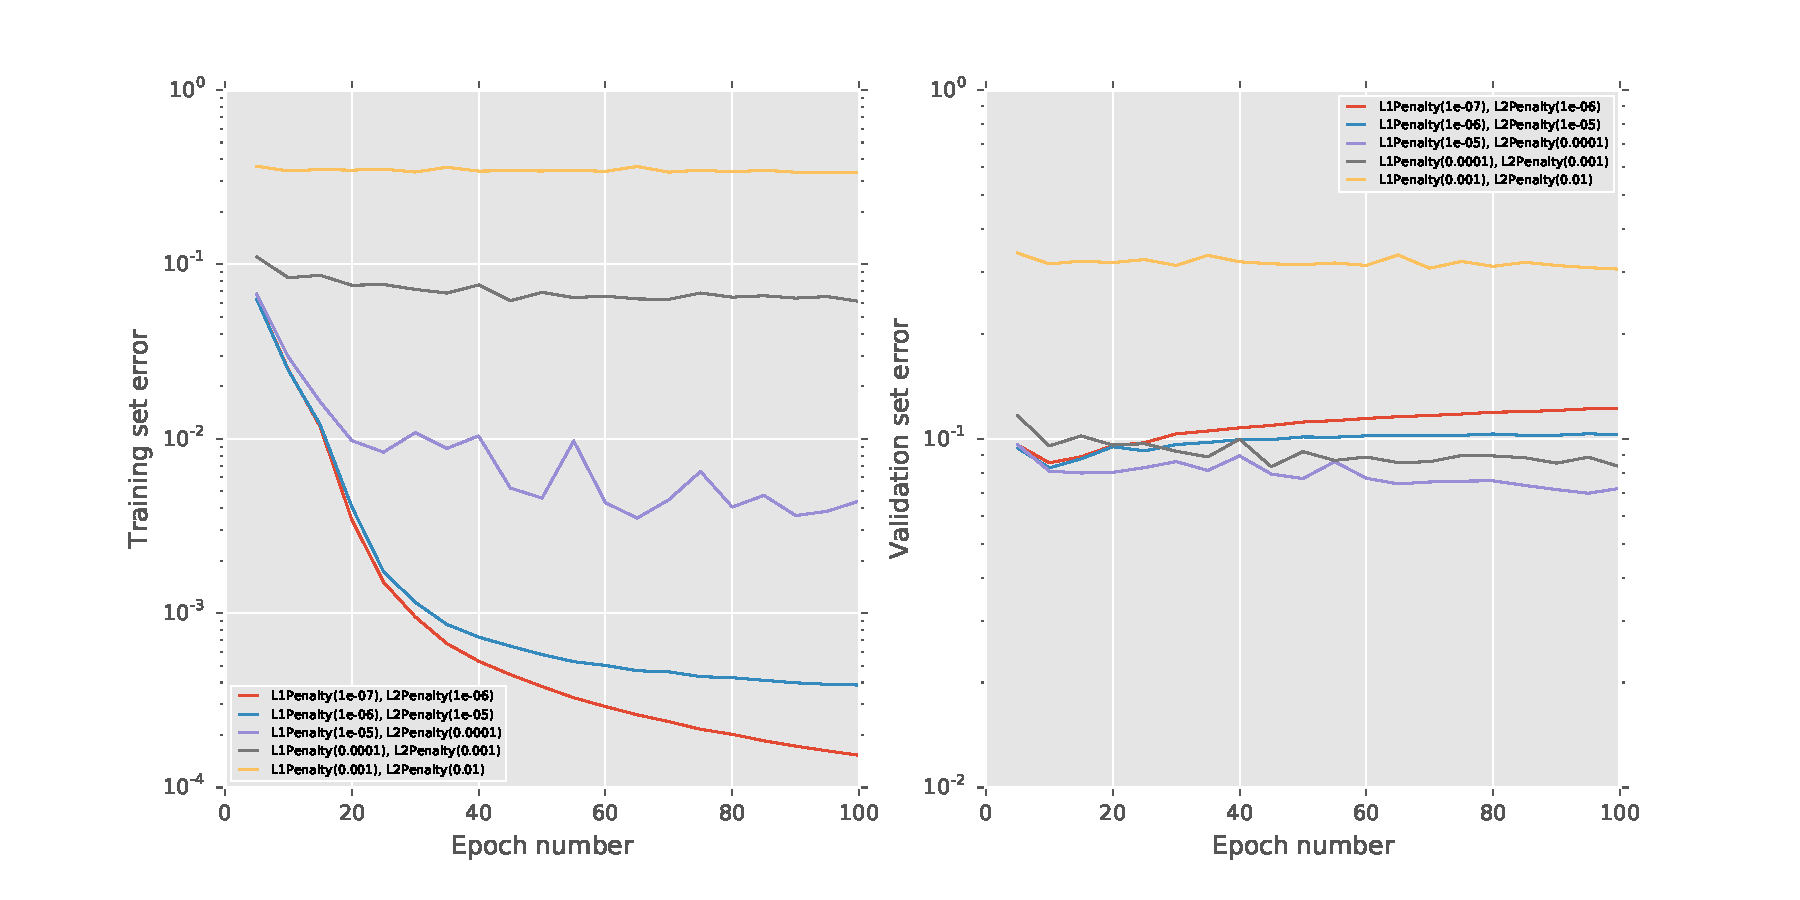
\includegraphics[width=1\textwidth]{L1_L2.pdf}
  \caption{training error and validation error for L1 and L2 combination method}
  \label{fg:L1_L2_combine}
\end{figure}

\begin{table}[htp]
\begin{center}
\begin{tabular}{ c  c c c c  c c} 
\hline
coeff\_L1 & coeff\_L2 &error(train) & error(valid) & acc(train) & acc(valid) & params\_penalty\\
\hline
\hline
None & None	&1.34e-04 & 1.22e-01 & 1.00e+00 & 9.79e-01 &0\\ 
1e-05 & None 	&1.64e-03 & 8.29e-02 & 1.00e+00 & 9.80e-01 &1.98e-02\\ 
None &1e-04	 &2.32e-03 & 7.57e-02 & 1.00e+00 & 9.81e-01 &1.56e-02\\ 
1e-05 &1e-04	 &4.39e-03 & 7.21e-02 & 1.00e+00 & 9.80e-01 &3.38e-02\\ 
\end{tabular}
\caption{Comparison between combined method and L1, L2 methods}
\label{tb:L1_L2_combine}
\end{center}	
\end{table}

\begin{figure}[htp]
\centering 
  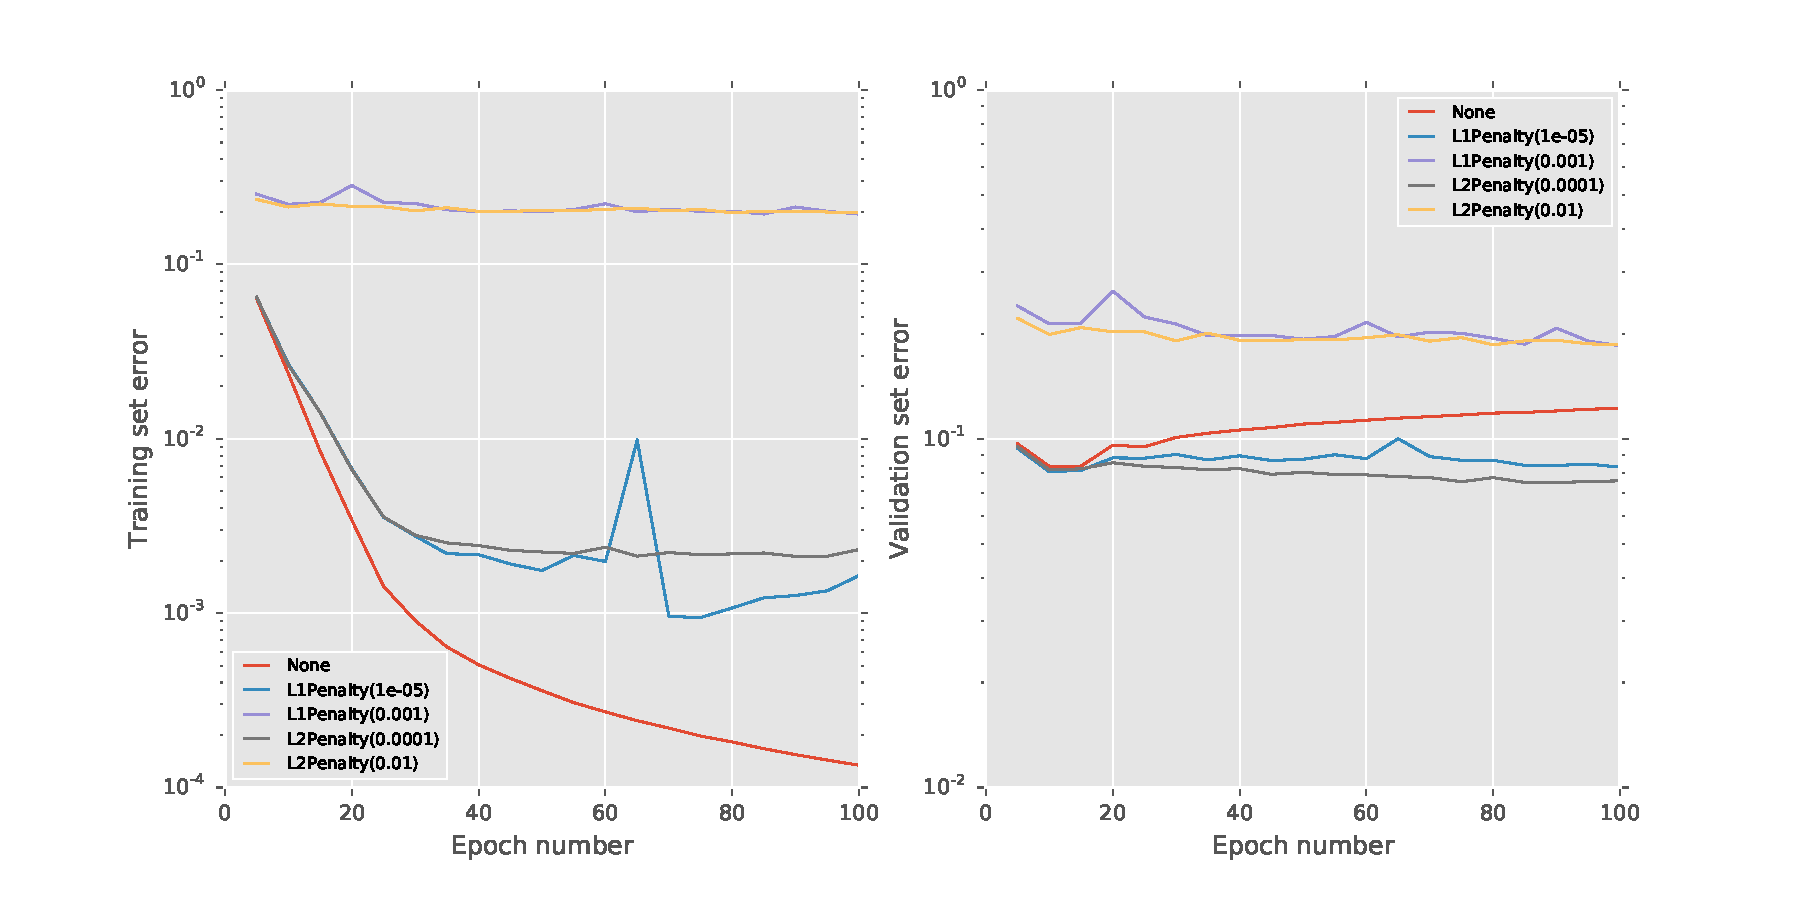
\includegraphics[width=1\textwidth]{baseline_L1_L2.pdf}
  \caption{training error and validation error for L1 and L2 penaly method}
  \label{fg:L1_L2_combine}
\end{figure}

\begin{figure}[htp]
\centering 
  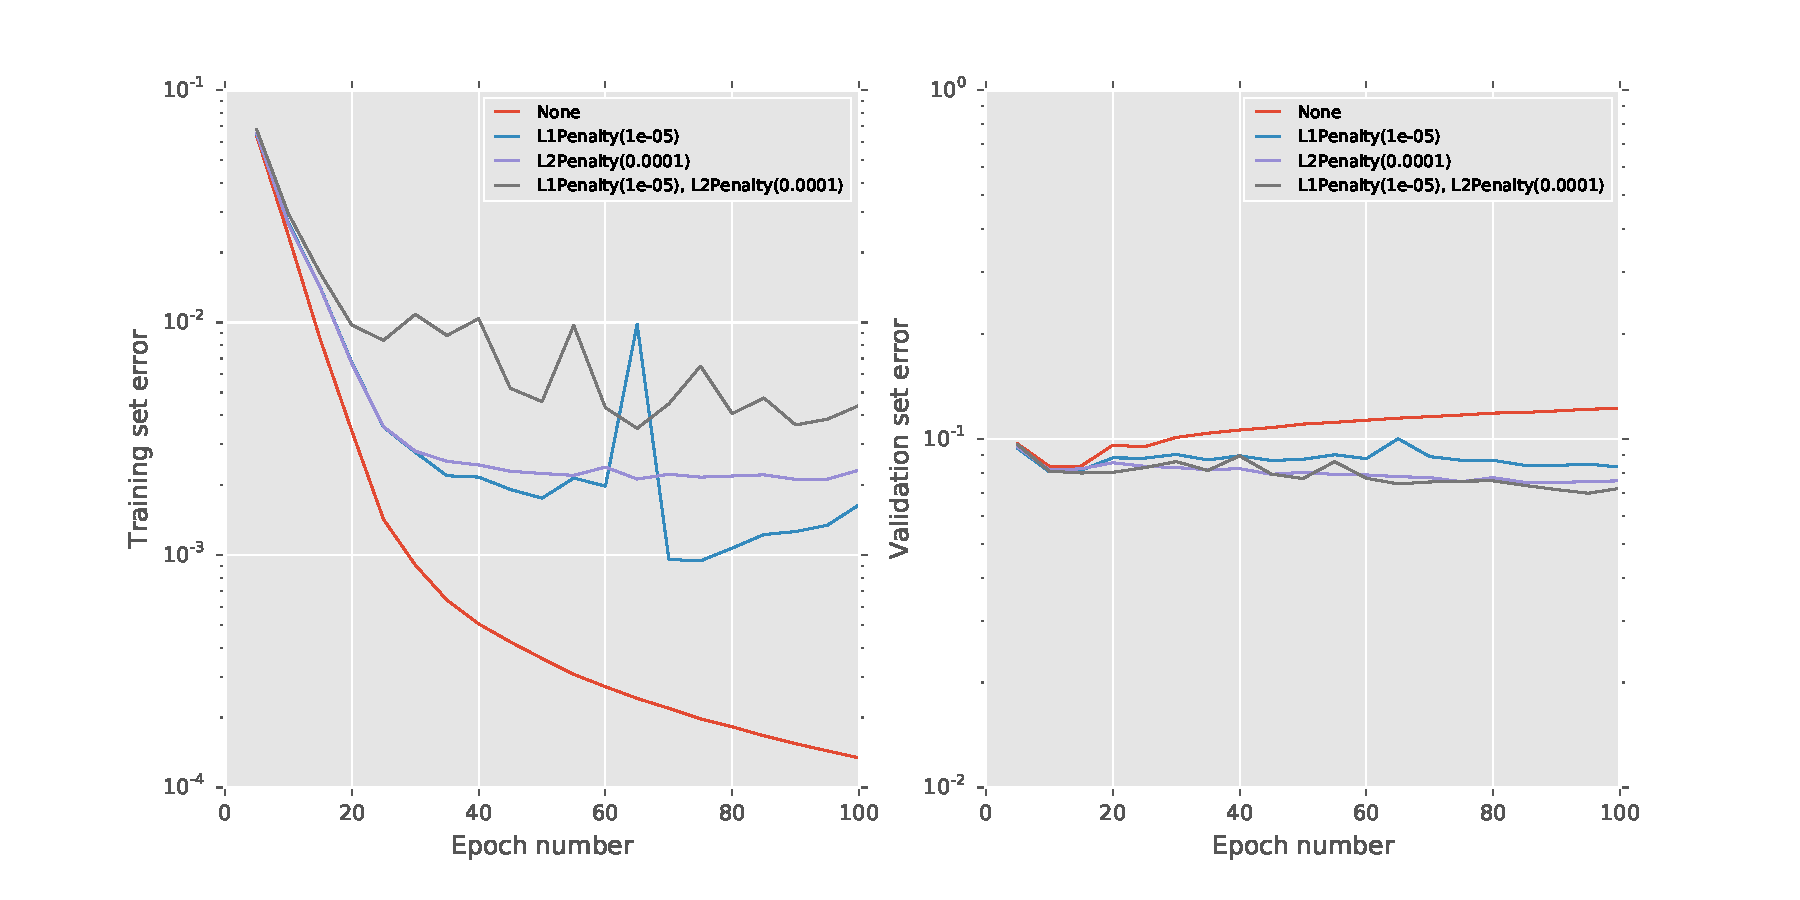
\includegraphics[width=1\textwidth]{L1_L2_with_all.pdf}
  \caption{Comparison between combining method, L1 and L2 penalty method}
  \label{fg:L1_L2_compare}
\end{figure}


\subsection{Discussion and Conclusion}
From the Table \ref{tb:L1_L2_combine}, it can be shown that the smallest validation error is achieved when coefficient for L1 is $1e-05$ and coefficient for L2 is $1e-04$. The parameters penalty is neither too high nor too lower so that the model will not overfitting nor underfitting. For larger coefficients the parameters penalty is too large so that the speed of learning is very slow. However, For smaller coefficients, the validation error starts to increase with the decreasing of training error, which indicates a overfitting problem. On reason for that could be the relatively small value of coefficients on L1 and L2 term so that the effects of penalty is minor.

In conclusion, the combining method of L1 and L2 weights methods do provide better performance on validation error though the difference is small. In consideration to the computational cost, it is not worthwhile to use L1 and L2 regularisation.

\newpage
\section{Data Augmentation}
\subsection{Experimental hypothesis}
Several ways was investigated to expand the training data such as rotating, zooming of existing data and elastic deformation \cite{Elastic}. In this experiment, we are going to find wether additional inputs generated from training data could provide better performance on validation set and how well do different ways of distortion perform on validation sets.
\subsection{Methodology}
In this section, the methodology of two ways of distortion is introduced.
\subsubsection{Random Zoom}
one quarter of training data will be randomly chosen to be zoomed by a factor of $\pm 0.2$. Then, theses distorted data will be added to the training set.
A function named {\bf random\_zoom} was developed. First, the indices of images to be zoomed was selected. Then, for each images, the zoom factor was chosen using uniform distribution in the range from $1.2$ to $0.8$. Then, if it's zoomed in, the dimension of the zoomed images will be larger than original dimension of $28\times 28 $. Therefore, the centeral $28 \times 28$ of pixels of zoomed images will be chosen to be the new images for training. Otherwise, the dimension of the zoomed images will be smaller than original dimension of $28 \times 28$. Therefore, the zoomed images will be added to the central of the new images to be training. Therefore, the dimensional size of the new image will be unchanged during zooming. Finally, the images was reshaped to the standard size for training. 
\subsubsection{Elastic Distortion}
In the case of handwriting recognition, \cite{Elastic} provides a way to provide similar uncontrolled oscillation of the hand muscles. A function named {\bf elastic\_deformation} was developed. Firstly, similar to {\bf random\_zoom}, a quarter of training data will be randomly selected for elastic deformation. It is generated first by random displacements fields. $\Delta x(x,y) = rand(-1, +1)$ and $\Delta y(x,y) = rand(-1, +1)$, where $rand(-1, +1)$ is a random number uniformly distributed between $-1$ and $+1$. Then, $\Delta x$ and $\Delta y$ is convolved with a Gaussian distribution with standard deviation $\sigma$ and then scaled by a factor of $\alpha$.

\subsection{Implementation and Results}
The final result for different type of augmentation was obtained by training each of them individually at first. Then, the results was shown by combining all the stats. The Table \ref{tb:aug} shows the results of error and accuracy for both training and validation sets.

\begin{table}[htp]
\begin{center}
\begin{tabular}{ c  c c c c  c c} 
\hline
Type &error(train) & error(valid) & acc(train) & acc(valid) \\
\hline
\hline
None & 1.34e-04 & 1.22e-01 & 1.00e+00 &9.79e-01 \\
 rotation	&2.21e-02 & 8.22e-02 & 9.93e-01 & 9.80e-01 \\ 
 Zoom  &8.00e-03 & 8.45e-02 & 9.98e+00 & 9.81e-01 \\ 
Elastic	 &5.71e-02 & 4.50e-02 & 9.83e+00 & 9.87e-01 \\ 
\end{tabular}
\caption{Performance of different ways of data augmentation}
\label{tb:aug}
\end{center}	
\end{table}






In the Figure \ref{fg:zoom_batch}, we can find that some of numbers is zoomed in and some of numbers is zoomed out. 
In the Figure \ref{fg:ela_batch}, we can find the impact of elastic deformation with different value of $\sigma$. The $\alpha$ is set to $34$ according to the authors \cite{Elastic}. The best $\sigma$ is chosen to be $4$ for training. The final training and validation results is shown in Figure.


\begin{figure*}[htp]
    \centering
    \begin{subfigure}[t]{0.45\textwidth}
        \centering
        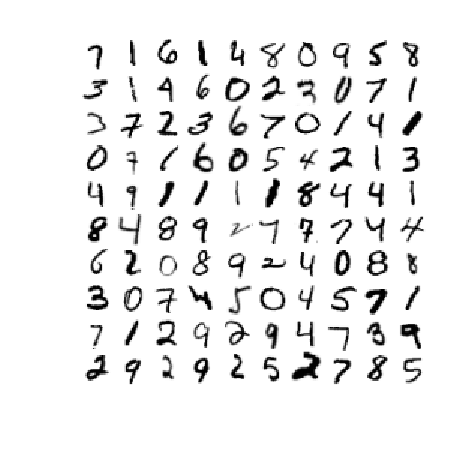
\includegraphics[height=3in]{zoom_org}
        \caption{Original}
    \end{subfigure}%
    ~ 
    \begin{subfigure}[t]{0.45\textwidth}
        \centering
        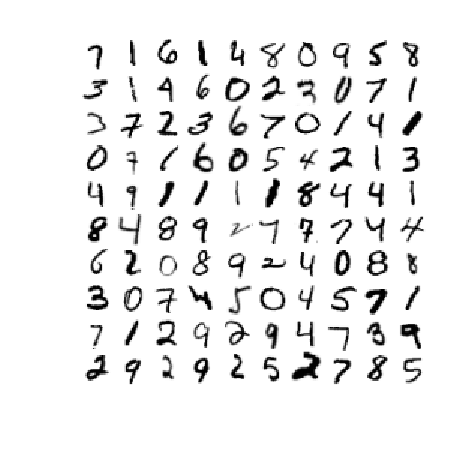
\includegraphics[height=3in]{zoom_img}
        \caption{Zoomed}
    \end{subfigure}
    \caption{Batch of images for zooming}
    \label{fg:zoom_batch}
\end{figure*}

\begin{figure*}[htp]
    \centering
    \begin{subfigure}[t]{0.45\textwidth}
        \centering
        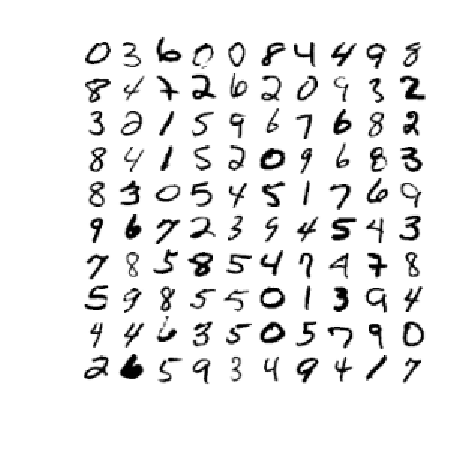
\includegraphics[height=2.8in]{ela_org}
        \caption{Original}
    \end{subfigure}
    ~ 
    \begin{subfigure}[t]{0.45\textwidth}
        \centering
        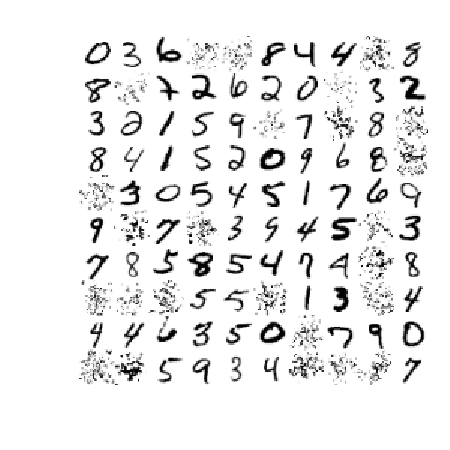
\includegraphics[height=2.8in]{ela_sig_1}
        \caption{$\sigma = 1$}
    \end{subfigure}
    \begin{subfigure}[t]{0.45\textwidth}
        \centering
        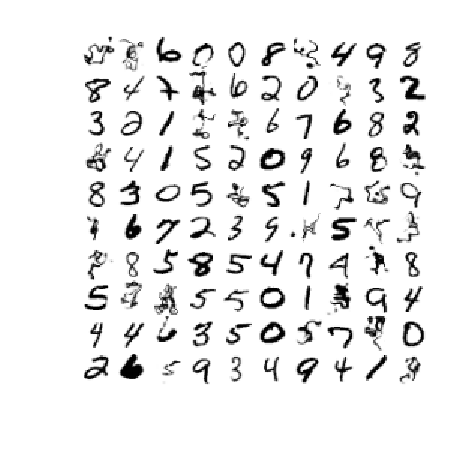
\includegraphics[height=2.8in]{ela_sig_2}
        \caption{$\sigma = 2$}
    \end{subfigure}
    ~ 
    \begin{subfigure}[t]{0.45\textwidth}
        \centering
        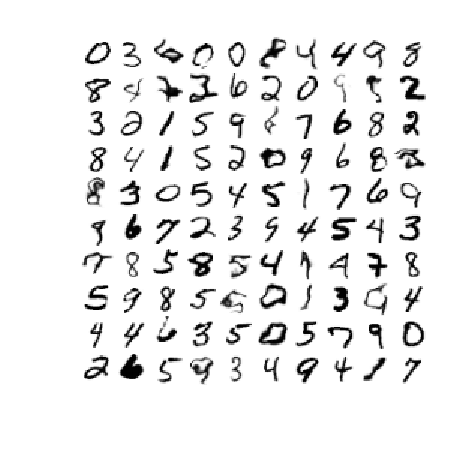
\includegraphics[height=2.8in]{ela_sig_3}
        \caption{$\sigma = 3$}
    \end{subfigure}
        \begin{subfigure}[t]{0.45\textwidth}
        \centering
        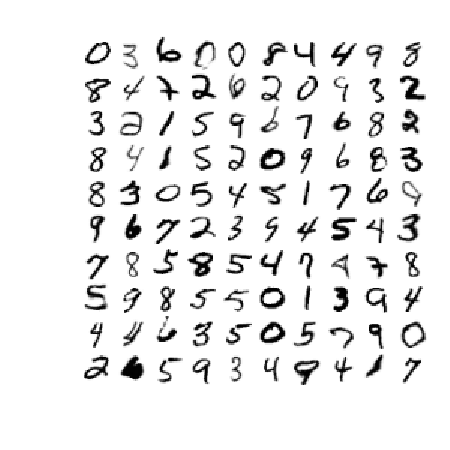
\includegraphics[height=2.8in]{ela_sig_4}
        \caption{$\sigma = 4$}
    \end{subfigure}
    ~ 
    \begin{subfigure}[t]{0.45\textwidth}
        \centering
        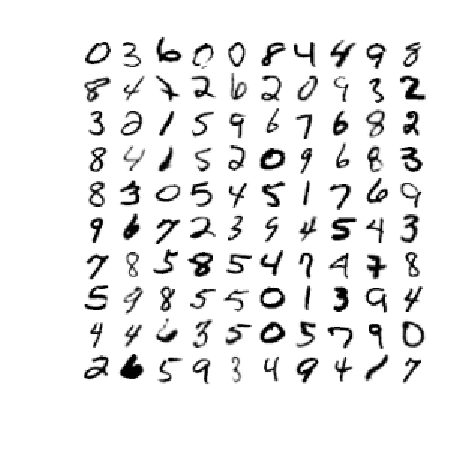
\includegraphics[height=2.8in]{ela_sig_5}
        \caption{$\sigma = 5$}
    \end{subfigure}
    \caption{Batch of images for elastic deformation}
    \label{fg:ela_batch}
\end{figure*}


\begin{figure}[htp]
\centering 
  \includegraphics[width=1\textwidth]{error_aug.pdf}
  \caption{training error and validation error for data augmentation}
  \label{fig:aug_error}
\end{figure}

\begin{figure}[htp]
\centering 
  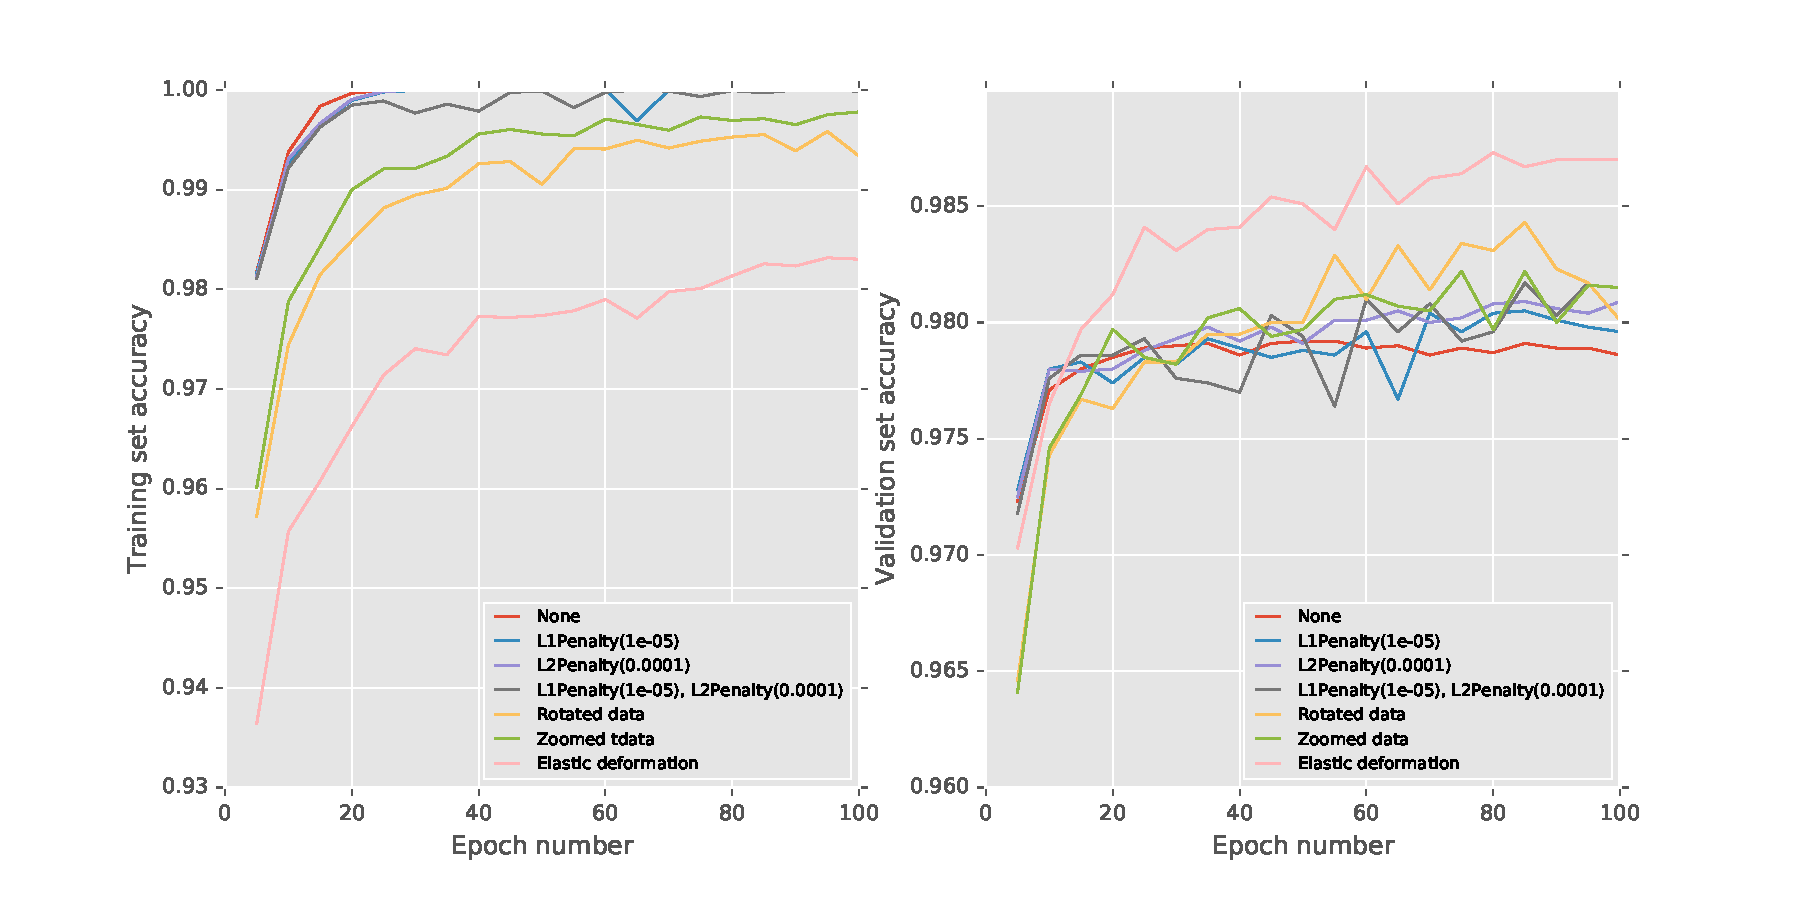
\includegraphics[width=1\textwidth]{acc_aug.pdf}
  \caption{training accuracy and validation accuracy for data augmentation}
  \label{fig:aug_error}
\end{figure}

\subsection{Discussion and Conclusion}
From the results above, it can be seen that by applying the method of  data augmentation, the overfitting is reduced since the training error is increased while the validation error is decreased. From the three ways of data augmentation, the elastic deformation has the best performance. It not only avoid overfitting the training data, but also fitting well on validation sets. 

The reason that the elastic deformation has the best performance is that it is a probably more realistic distortion compared to other methods. That means the additional data is more similar to the validation data. The more similar the artificial created data is, the better result the model will be.

In conclusion, we found that the additional augmented data can provide better performance. Elastic deformation has the best performance of all. 

\newpage

\section{Convolution layer}
\subsection{Experimental hypothesis}
In this section, a convolution layer and a max-pooling layer was developed. The hypothesis is to evaluate the impact of the max-pooling layer on the convolutional neural network (CNN).
\subsection{Methodology}
\subsubsection{Convolution layer}
The inputs Assuming the inputs was a 4D tensor (batch size, number of input channels, input dimension 1, input dimension 2), the output for each unit in the next hidden layer is calculated by:
\begin{equation}
	h_{i,j} = \Theta(\sum_{k=0}^{m-1}\sum_{l=0}^{m-1}w_{k,l}x_{i+k,j+l}+b)
\end{equation}
where $i,j$ is the indices for the row and column, $\Theta$ is the activation function such as the $ReLU$, $Sigmoid$ or the $hyperbolic$ $tangent$ function, $w_{k,l}$ are elements of the shared $m \times m$ weight matrix {\bf w}.

For the back propagation, the gradient with respect to the inputs is:
\begin{equation}
	\delta_n^{(x)} = \frac{\partial J}{\partial x_n} = \frac{\partial J}{\partial y}\frac{\partial y}{\partial x_n} = \sum_{i=0}^{m} \frac{\partial J}{\partial y_{n-i}}\frac{\partial y_{n-i}}{\partial x_n} = \sum_{i=0}^{m}\delta_{n-i}^{(y)}w_i = \Big(\delta^{(y)}*flip(w_i)\Big) [n]
\end{equation}
the gradient with respect to the kernels is:
\begin{equation}
\frac{\partial J}{\partial w_i} = \frac{\partial J}{\partial y}\frac{\partial y}{\partial w_i} = \sum _{j=0}^{d-m+1} \frac{\partial J}{\partial y_{j}}\frac{\partial y_{j}}{\partial w_i} = \sum_{j=0}^{d-m+1}\delta_j^{(y)}x_{j+i} = \Big(\delta^{(y)} * flip(x) \Big)[i]
\end{equation}
where $d$ is the input dimension. 
\subsubsection{Pooling Layer}
The max-pooling layer is investigated in this section. It subsamples a feature map and reduce its size. In this experiment, it reduces a set of $2\times 2$ regions to a single unit. The way to reduce is max-out which means the maximum among the $4$ units becomes the output of the pooling layer. In forward propagation, the output of the pooling layer is:
\begin{equation}
	y(x) = max(x)
\end{equation}

for back propagation,
\[ \frac{\partial y}{\partial x_i} =
  \begin{cases}
    1       & \quad \text{if } x_i =\text{ max} (x)\\
    0  & \quad \text{otherwise }\\
  \end{cases}
\]
\begin{equation}
	\frac{\partial J}{\partial x} = \frac{\partial J}{\partial y_n}\frac{\partial y_n}{\partial x} = \delta^{(y)}\frac{\partial y}{\partial x}
\end{equation}
\subsection{Implementation and Results}
\subsubsection{Convolution layer}
For the convolution layer, the class {\bf ConvolutionalLayer} was developed. The method {\bf fprop} was developed for the forward propagation. The inputs image is $2$-dimensions ($x$, $y$). The input of the method is variable {\bf inputs}, a $4$-dimensional tensor (batch size, number of input channels, $x$, $y$). The output of the method is variable {\bf outputs}, a $4$-dimensional tensor (batch size, number of output channels, $x$ - $m$ + 1, $y$ - $m$ +1), where $m$ is the the 2-dimensional kernel ($m \times m$) size, with no-padding and unit strides. 

For the method of {\bf bprop}, it is used to calculate the gradients with respect to the inputs. The input arguments are {\bf inputs}, {\bf outputs} and a 4-dimensional tensor {\bf grad\_wrt\_outputs} (batch size, number of output channels, $x$ - $m$ +1, $y$ - $m$ + 1). The return value of the method is {\bf grad\_wrt\_inputs} which is an 4-D tensor (batch size, number of input channels, $x$, $y$). 

For the method of {\bf grads\_wrt\_params}, the inputs arguments are {\bf inputs} and {\bf grad\_wrt\_outputs}. The output is a list of arrays of gradients with respect to the layer parameters. The list contains  {\bf grads\_wrt\_kernels} contains {\bf grads\_wrt\_biases}.

\subsubsection{Pooling Layer}
For the max-pooling layer, the class {\bf MaxPoolingLayer} was developed. It has internal arguments {\bf pool\_size\_1} and {\bf pool\_size\_2}. In this implementation, the default value for both of them is $2$.

For the method of {\bf fprop}, the inputs of the method is {\bf inputs}, which is a 4-dimensional tensor (batch size, number of channels, x, y). the output tensor is also 4-dimensional but the size of each size of the output image is halved. since both of the pool size is $2$.

For the method of {\bf bprop}, the inputs of the method  are {\bf inputs}, {\bf outputs} and {\bf grads\_wrt\_outputs}. The return tensor is {\bf grads\_wrt\_inputs}.

\subsubsection{Results}

The code is implemented in the file {\bf CW2\_Q3.ipynb}. The total number of epochs is limited to $30$ due to high time-consumption of training. The baseline was a model with two affine layer using $ReLu$ as the activation function. The plots of error and accuracy on training and validation sets was shown in Figure \ref{fg:cnn_error} and Figure \ref{fg:cnn_acc}. The plot of error is log-scaled. The Table \ref{tb:cnn} shows the value of the performance for every model. 

\begin{table}[htp]
\begin{center}
\begin{tabular}{ c c c c c  c c} 
\hline
Type &error(train) & error(valid) & acc(train) & acc(valid) \\
\hline
\hline
Baseline & 8.57e-04 & 1.02e-01 & 1.00e+00 &9.80e-01 \\
cnn\_only	&1.28e-04 & 1.29e-01 & 1.00e+00 & 9.80e-01 \\ 
cnn\_pooling &2.67e-04 & 8.91e-02 & 1.00e+00 & 9.84e-01 \\ 
\end{tabular}
\caption{Performance on experiment of convolution layer }
\label{tb:cnn}
\end{center}	
\end{table}

\begin{figure}[htp]
\centering 
  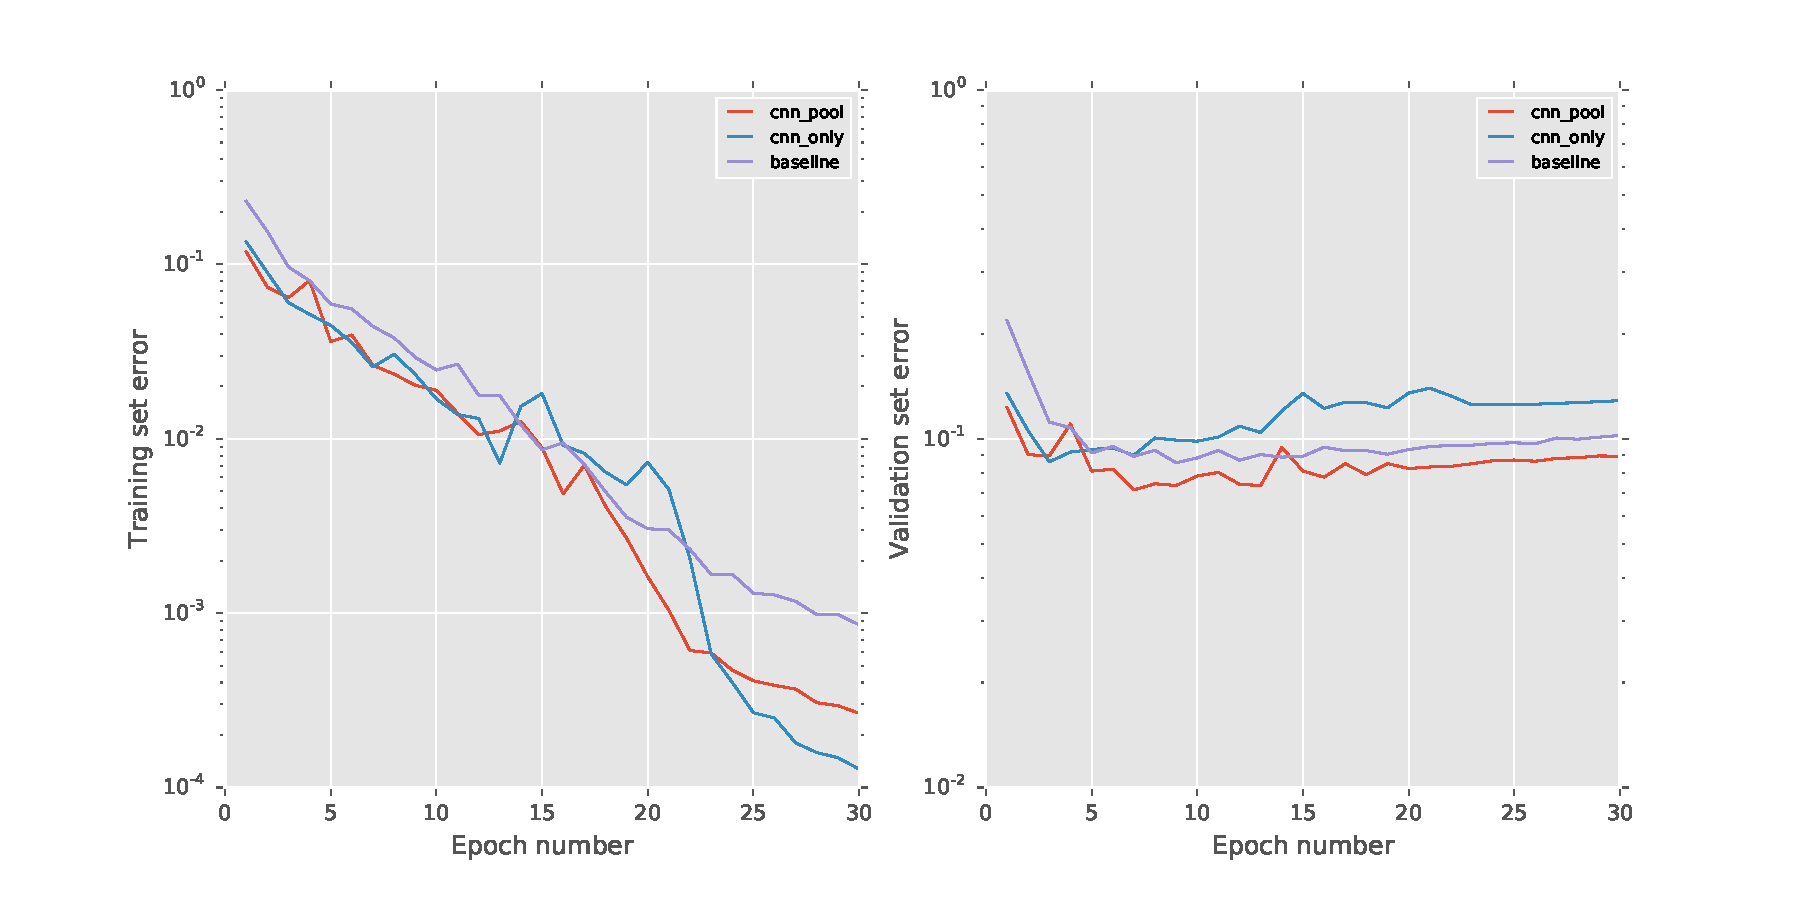
\includegraphics[width=1\textwidth]{cnn_error.pdf}
  \caption{training error and validation error for CNN}
  \label{fg:cnn_error}
\end{figure}

\begin{figure}[htp]
\centering 
  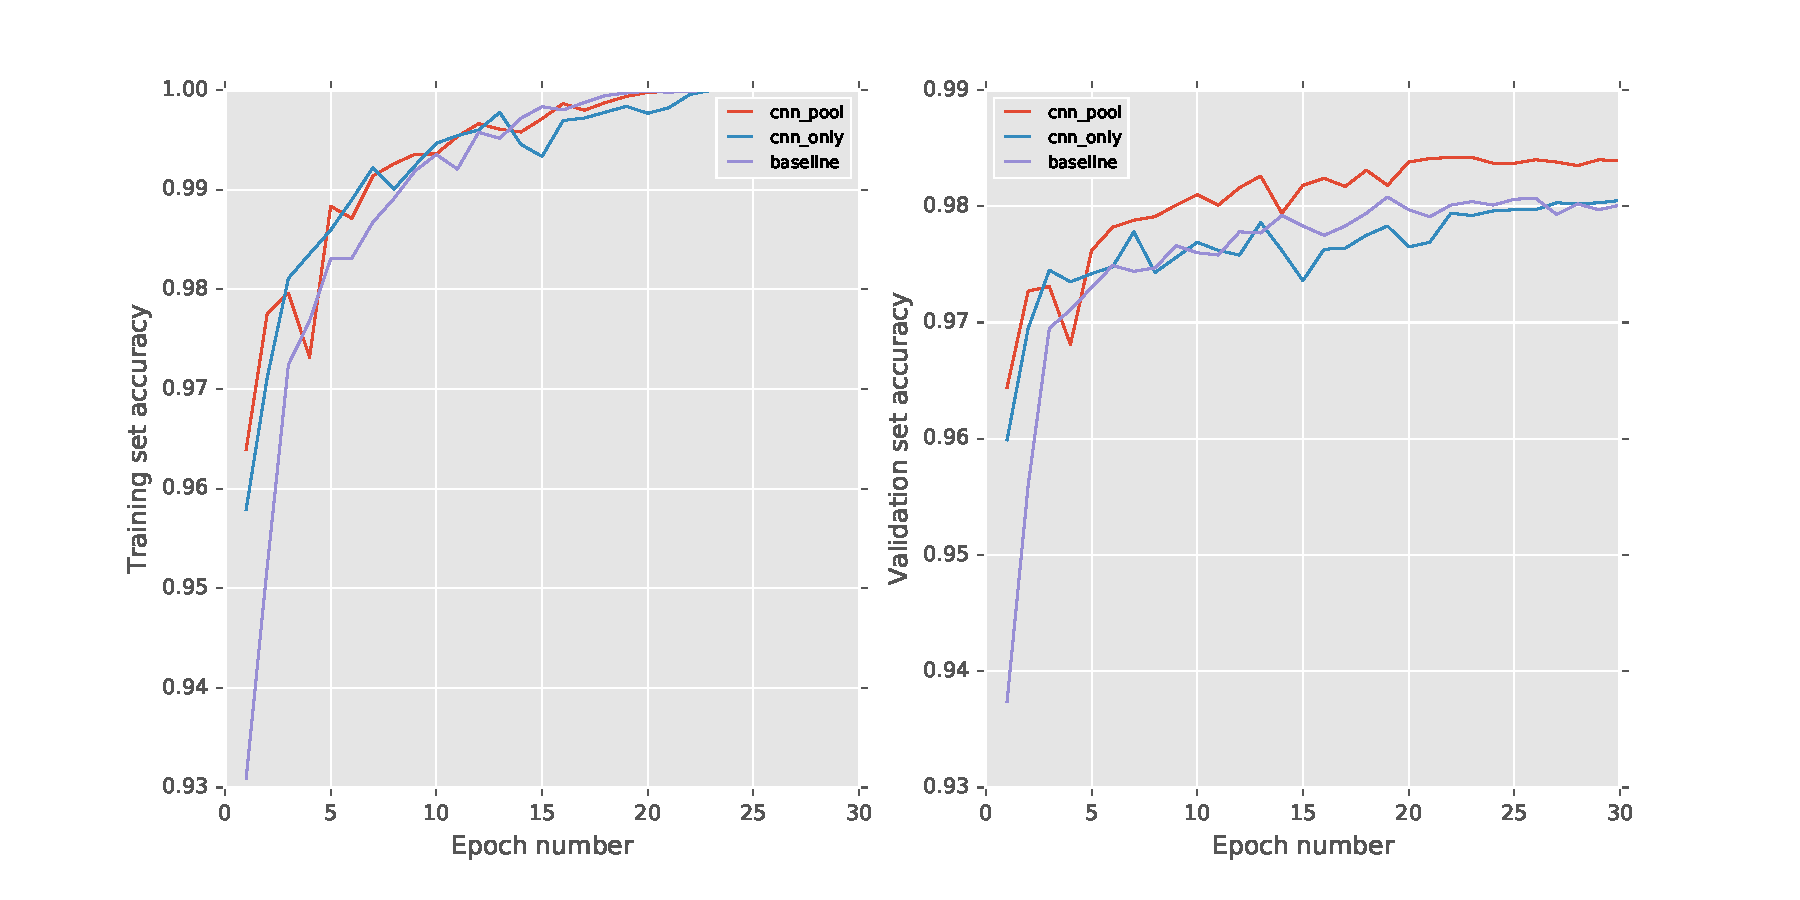
\includegraphics[width=1\textwidth]{cnn_acc.pdf}
  \caption{training accuracy and validation accuracy for CNN}
  \label{fg:cnn_acc}
\end{figure}

\newpage
\subsection{Discussion and Conclusion}
The plot illustrates that the CNN with pooling layer has higher accuracy and lower error on the validation sets, while it has lower error in training sets. Therefore, it reduces the overfitting. 

Since max pooling operation replace the outputs of convolution layer at a certain location with a summary statistic of pixels nearby, it is helpful to make the representation become approximately invariant to small translation of the input \cite{Goodfellow-et-al-2016-Book}. 

In the MNIST classification problem, we care more about whether some feature is present rather than where it is. The use of pooling layer can be assumed to add an infinity strong prior that the feature learned by the neural network must be invariant to small translations. It can improve the efficiency of the network when this assumption is correct \cite{Goodfellow-et-al-2016-Book}. 

Another benefits of pooling layer is that it has fewer pooled features which helps to reduce the number of kernel parameters in later layers. 

In conclusion, a max-pooling layer can improve the performance of a convolutional neural network in both accuracy, error but also in reducing overfitting.
\newpage
\printbibliography
\end{document}